\documentclass[11pt,a4paper,titlepage,openright]{report}
\usepackage[utf8]{inputenc}
\usepackage[T1]{fontenc}
\usepackage[french]{babel}
\usepackage[top=1.5cm, bottom=4cm]{geometry}
\usepackage{fancyhdr, graphicx, array, hyperref}
\usepackage{glossaries}

\pagestyle{fancy}

\title{\textsc{\textbf{Plan projet\\Interpréteur du langage LIR}}}
\date{}
\author{Nicolas \textsc{Caminade} \and Sylvan \textsc{Courtiol} \and
    Pierre \textsc{Debas} \and Heïa \textsc{Dexter} \and Lucàs
    \textsc{Vabre} }
\begin{document}
    \lhead{\leftmark}
    \rhead{
        
\includegraphics[width=2cm]{img/logoiut}
    }

    \cfoot{\thepage}
    \headheight = 2cm
    \headsep = 0.5cm

    \begin{titlepage}
        \fontfamily{pag}\selectfont

        \begin{center}\normalsize
            \MakeUppercase{IUT de Rodez \hfill Département informatique
                \hfill INFO1 2020-2021}
        \end{center}
        \vspace*{0.1cm}
        \hrule
        \vspace*{0.2cm}
        \begin{flushright}
            
\includegraphics[width=4cm]{img/logoiut}
        \end{flushright}
        \vspace*{2cm}
        \begin{flushright}\Huge
            \textsc{\textbf{Plan projet\\Interpréteur du langage LIR}}
        \end{flushright}
        \hrule
        \begin{flushleft}
            \MakeUppercase{Projet proposé par Frédérique Barrios}
        \end{flushleft}
        \vspace*{2cm}
        \begin{center}\Large
            Nicolas \textsc{Caminade}, Sylvan \textsc{Courtiol},\\
            Pierre \textsc{Debas}, Heïa \textsc{Dexter}, \\
            Lucàs \textsc{Vabre}
        \end{center}
        \vfill
        \begin{center}\normalsize
            \MakeUppercase{Projet tuteuré --- Semestre 2}
        \end{center}
    \end{titlepage}


    % Sommaire
    \renewcommand{\contentsname}{Sommaire}
    \tableofcontents

    \chapter*{Introduction}
    \Large
    Dans le cadre des projets tuteuré du semestre 2 de première année de
    DUT informatique de l’année 2020-2021, le sujet de l’Interpréteur LIR
    a été proposé par F. Barrios, un des enseignants de l’IUT de Rodez.
    \\Ce document a pour but de rassembler les informations fondamentales
    relatives à la gestion du projet. Ce plan projet est un document de
    référence du projet qui sera complété tout au long de son avancement.

    \normalsize
    \chapter{Présentation du projet}
    \section{Définition générale du besoin : l'Interpréteur LIR}
    L’Interpréteur LIR est un interpréteur d’un langage de programmation
    simple, il sera nommé LIR pour Langage IUT de Rodez.
    Un interpréteur est un automate enchaînant les tâches suivantes :
    analyse lexico-syntaxique d’une ligne de commande puis interprétation.
    \\Une ligne entrée par un utilisateur sera donc : soit une commande à
    exécuter immédiatement, soit une ligne de programme à mémoriser pour
    une exécution ultérieure. Une ligne de programme se distinguera d'une
    ligne de commande par le fait qu'elle sera toujours précédée d'un
    "numéro d'ordre" appelé aussi "étiquette".

    \section{Cahier des charges}
    Le document en annexe fourni par la maîtrise d’ouvrage (MOA) définit
    l’interpréteur attendu avec les éléments du Langage IUT de Rodez, la
    syntaxe des instructions de programmation et des commandes générales
    attendues dans le logiciel final. Le document précise également le
    comportement attendu de l’interpréteur lors de son utilisation suivi
    d’un exemple d’une session sous cet interpréteur LIR.

    \section{Définitions et acronymes}
        \paragraph{Analyse syntaxique :}
        La vérification de la conformité aux contraintes syntaxiques
        définies par une grammaire.

        \paragraph{Analyse lexicale :}
        L’identification des éléments du vocabulaire d’un langage dans
        une description textuelle (scanning) et la recherche des unités
        lexicales (lexèmes).

        \paragraph{Grammaire :}
        Contraintes syntaxiques définissant les constructions correctes
        (autorisées) d’un langage.

        \paragraph{Interpréteur :}
        Programme capable d’analyser les instructions d’un langage
        (évolué) et de les exécuter directement.

        \paragraph{Langage :}
        Outil de description et d’expression.

        \paragraph{Langage IUT de Rodez (LIR)}

        \paragraph{Sémantique :}
        Étude du sens des unités linguistiques et de leurs combinaisons.
        \\Aspect de la logique qui traite de l'interprétation et de la signification des systèmes formels, par opposition à la syntaxe, entendue comme l'étude des relations formelles entre formules de tels systèmes (d’après le dictionnaire Larousse).

        \paragraph{Syntaxe :}
        Partie de la grammaire qui décrit les règles par lesquelles les unités linguistiques se combinent en phrases. En logique, étude des relations formelles entre expressions d'un langage (d’après le dictionnaire Larousse).
        \\Aussi, la syntaxe est spécifiée par des grammaires et des notations formelles.

        \paragraph{Vocabulaire :}
        Symboles de base utilisés dans un langage.

    \section{Charte de projet}
    \subsection{Objectifs du projet}
    Réaliser un interpréteur capable d'exécuter un script ou une série
    d'instructions dans le langage LIR avec les outils et connaissances
    et mis à disposition par l’IUT de Rodez.

    \subsection{Périmètre du projet}
    Ce projet est doit être mené jusqu'à obtention d’un interpréteur
    capable d’exécuter toutes les commandes précisées dans le cahier des
    charges fourni.

    \subsection{Demandes hors périmètre}
    Il n’y a pas de demandes hors périmètre.

    \subsection{Principaux livrables identifiés}
    \paragraph{Livrables :} plan projet, dossier de projet, CD (de
    préférence un dossier compressé plutôt qu’un CD) contenant les codes
    exécutables les fichiers de données, les codes sources et la version
    numérique du dossier et le manuel utilisateur.

    \paragraph{Définition du cadre}
    \subparagraph{Coût :} À définir par le chef de projet (P. Debas).
    \subparagraph{Délais :} Deux dates butoirs identifiées.
        \begin{itemize}
            \item Remise du projet le vendredi 28 mai 2021.
            \item Soutenance du projet la semaine du 7 juin 2021.
        \end{itemize}

    \subparagraph{Qualité :}
    Projet codé en Java dans les respects des conventions et bonnes
    pratiques.

    \subsection{Les acteurs du projet}

    \begin{center}
        \begin{tabular}{rl}
            L'équipe MOE :        & N. CAMINADE, S. COURTIOL, \\
                                  & P. DEBAS, H. DEXTER,      \\
                                  & L. VABRE                  \\
            La MOA :              & F. Barrios                \\
            Le contrôle qualité : & F. Barrios et J. Accot    \\
        \end{tabular}
    \end{center}

    \subsection{Autres moyens et ressources}
    Pas de moyens ou ressources supplémentaires.

    \subsection{Conditions d’acceptation}
    Pas d’exigence ou de contraintes supplémentaires.

    \subsection{Principaux risques identifiés et politique de gestion des risques}
    Si possible tous les membres du groupe auront les mêmes droits sur
    les fichiers communs. En conséquence chaque membre du groupe ne doit
    pas donner des droits sur ces fichiers à une personne extérieure au
    projet (autre que MOA). Cf. Gestion de la configuration (produit par
    S. Courtiol).
    \\Des sauvegardes du dépôt GitHub (contenant toutes les données du
    projets) seront effectuées régulièrement (fréquence à définir) par le
    gestionnaire de configuration. Toutes données qui ne sont pas dans le
    dépôt sont à la responsabilité de chacun. Cf. Gestion de la
    configuration (produit par S. Courtiol).

    \section{Étude générale du besoin}
    \paragraph{Diagramme de cas d'utilisation général de l'Interpréteur LIR}
    comprenant un acteur (le programmeur) et cinq cas d'utilisation
    identifiés comme suit :
    \\

    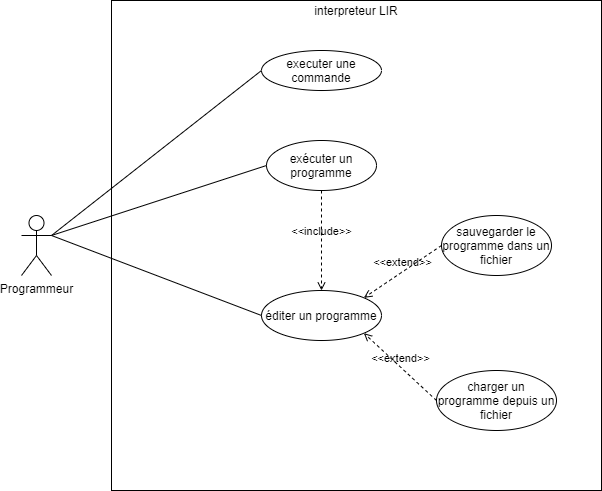
\includegraphics[width=\linewidth]{img/diagrammeDeCasUtilisation}

    \subsection{Les acteurs}
    \paragraph{Programmeur :} % TODO à détailler
    Lorem ipsum dolor sit amet, consectetur adipiscing elit. Mauris nec ultrices velit. Curabitur convallis non ipsum malesuada fringilla.

    \subsection{Résumés de cas d'utilisation}
    \subsubsection{Exécuter une commande}
    \subsubsection{Exécuter un programme}
    \subsubsection{Éditer un programme}
    \subsubsection{Sauvegarder le programme dans un fichier}
    \subsubsection{Charger un programme depuis un fichier}

    %TODO: à ajouter

    \subsection{Récits d'utilisation (user stories)}

    %TODO: à ajouter

    \chapter{Organisation du projet}
    \section{Présentation du cycle de vie itératif} % TODO Finir rédaction
    Le modèle de cycle de vie choisi est le modèle itératif.
    \\Présentation du cycle et ses conséquences sur l’organisation.

    Pour développer l’Interpréteur LIR, le modèle de cycle de vie itératif a été choisi. Ce modèle de développement de logiciel consiste en une succession de cycles de spécification, de conception, de réalisation et de tests, le but est d’enrichir et de « remodeler » des prototypes du logiciel successifs. Par conséquent, une version du logiciel sera un « dernier prototype ».
    \\La gestion du risque va entraîner la mise en place d’un noyau architectural avec des fonctions indispensables du logiciel dès les deux premières itérations. Les itérations suivantes apporteront des corrections et de nouvelles fonctions au logiciel.
    \\Les versions successives des prototypes permettent de matérialiser l’avancement et d’éviter « l’effet tunnel » sur le projet. Ces prototypes (versions 0.x) entretiennent la motivation des différents acteurs du projet : l’équipe MOE, la MOA.
    \\Le principe fondamental à chaque début d’itération est de ne spécifier en détail que les fonctionnalités nécessaires pour cette itération. Ainsi la prise en compte d’évolutions du besoin reste possible jusqu’à la dernière itération. De même le « refactoring » de la conception (largement facilité par les outils) a lieu à chaque étape pour intégrer des évolutions et des ajouts. Le but étant bien sûr de fabriquer le logiciel adapté au besoin en laissant la possibilité de « mûrir » au cours du temps.
    \\Ce type de cycle implique une taille homogène de l’équipe et une polyvalence des équipiers.

    \section{Répartition des rôles}
    Rôles des membres de l’équipe impliqués dans le projet jusqu'au mois de mai 2021 :
    \begin{center}
        \begin{tabular}{rl}
            Chef de projet MOE            & Pierre Debas      \\
            Secrétaire de projet          & Heïa Dexter       \\
            Gestionnaire de configuration & Sylvan Courtiol   \\
            Développeur                   & Nicolas Caminade  \\
            Développeur                   & Lucàs Vabre       \\
        \end{tabular}
    \end{center}

    \section{Plan communication}
    \subsection{Localisation géographique des intervenants}
    L'équipe MOE, la MOA et les contrôleurs qualités sont basés sur Rodez (12).
    \\La MOA, les contrôleurs qualités, H. Dexter sont basés sur Rodez (12), S. Courtiol sur Luc-La-Primaube à côté de Rodez (12), P. Debas est basé à la fois sur Rodez et à Albi (81), L. Vabre sur Gages (12) et N. Caminade sur Rodez et Moncaut (47).

    \subsection{Moyens de communication utilisés}
    Les communications formelles sont effectuées via les mails de l’IUT (généralement par le chef de projet) avec les autres membres du projet en CC.
    \\Serveur Discord spécifique au projet pour communication écrite ou vocale de la MOE.
    \\Cf. le document Configuration interpréteur du langage LIR produit par le gestionnaire de configuration (S. Courtiol).

    \subsection{Réunions projets MOE}
    Les réunions projet MOE seront hebdomadaires voire bi-hebdomadaires et dans le contexte de la crise sanitaire elles se dérouleront en distanciel via Discord (vocal, visio-conférence). Seront prévue des réunions courtes de 20 minutes et des réunions longues de 1h30.
    \\Ces réunions auront pour objectif de faire le point sur l’avancement du projet, le respect des objectifs fixé sur la période et de fixer les prochains objectifs à remplir d’ici la prochaine réunions. Aussi ces réunions seront l’occasion de faire part de difficultés éventuelles rencontrées par les membres de l’équipe au cours de la semaine et de communiquer les informations sur les prochaines rencontres avec la MOA.
    \\Les comptes-rendus seront rédigés par la secrétaire de projet (H. Dexter) et diffusés sur le serveur Discord de l’équipe sous format texte.

    \subsection{Comités de Pilotage}
    Les comités de pilotage rassembleront la MOA et toute l’équipe de MOE. Les COPIL seront dirigé par le chef de projet éventuellement assisté par le secrétaire.
    \\La fréquence des COPIL est au mieux hebdomadaire et d’une durée d’une demi-heure à trois quarts d’heure selon l’avancement du projet.
    Les comptes-rendus des COPIL seront rédigés par l’actuelle secrétaire de projet (H. Dexter) et diffusés le lendemain à la MOE du projet.


    \section{Assurance qualité}
    \subsection{Normes et standards de travail à observer (formalisme de modélisation, méthodes de contrôle, méthodes de développement, cycle de vie, conventions de code…)}
    % TODO: À définir
    \subsection{Manuel qualité et démarche qualité à observer (suivant la politique qualité de l’organisation), suivi et contrôle qualité (organisation, fréquence, participants).}
    % TODO: À commencer


    \section{Ressources matérielles et logicielles}
    % principaux matériels, réseaux, systèmes d’exploitation, sites intranet-internet (wiki, gestionnaire d’incident, référentiel…) et outils de génie logiciel utilisés.

    % TODO: ajouter le doc de Sylvan

    \chapter{Pilotage du projet}
    \section{Cycle de vie itératif}
    Pour développer l’Interpréteur LIR, le modèle de cycle de vie itératif a été choisi. Ce modèle de développement de logiciel, rappelons-le, consiste en une succession de cycles de spécification, de conception, de réalisation et de tests, le but est d’enrichir et de « remodeler » des prototypes du logiciel successifs. Par conséquent, une version du logiciel sera un « dernier prototype ».
    \\Si le choix de modèle de cycle de vie s'est porté sur le modèle itératif, c'est parce qu'il s'agit d"un modèle "réaliste" et possible à mettre en place dans le cadre des projets tuteurés :

    \begin{itemize}
        \item Une limitation de "l'effet tunnel" pour une meilleure dynamique et motivation des équipes (MOA et MOE).
        \item Une meilleure acceptation des changements grâce aux prototypes.
        \item Une meilleure gestion des risques.
        \item Est adapté pour une équipe de cinq personnes polyvalentes.
        \item Le principe d'itérations où seules les fonctionnalités nécessaires sont spécifiées en détail en début d'itération ce qui permet une évolution du besoin.
    \end{itemize}

    \section{Estimation initiale}
    \section{Planification prévisionnelle initiale}
    \section{Durée et ordonnancement des principales tâches et itérations}
    \section{Identification des premiers jalons}
    \section{Calendrier prévisionnel}
    \section{Organisation des réunions projets et comités de pilotage}
    \section{Suivi du projet par période}
    Pour chaque période :
    \subsection{Suivi d’avancement et mesure des écarts par rapport au prévisionnel revu lors de la période précédente}

    \subsection{Synthèse par "tableau de bord"}

    \subsection{Résultats des tests et recette de prototype de la période}

    \subsection{Résultats des revues/suivis/contrôles qualité de la période}

    \subsection{Identification des principaux écarts et problèmes constatés, solutions possibles}

    \subsection{Propositions de modification de la planification prévisionnelle pour tenir compte des corrections à apporter}

    \subsection{Comptes-rendus des réunions projets de la période}

    \subsection{Compte-rendu du comité de pilotage de la période}

    \subsection{Planification prévisionnelle révisée pour les périodes suivantes (en fonction des décisions prises)}


    % TODO: Glossaire

    % TODO: Inclure CdC, GestionConfiguration, Résumés de Cas d'utilisation, Récits d'utilisation

    \appendix
    %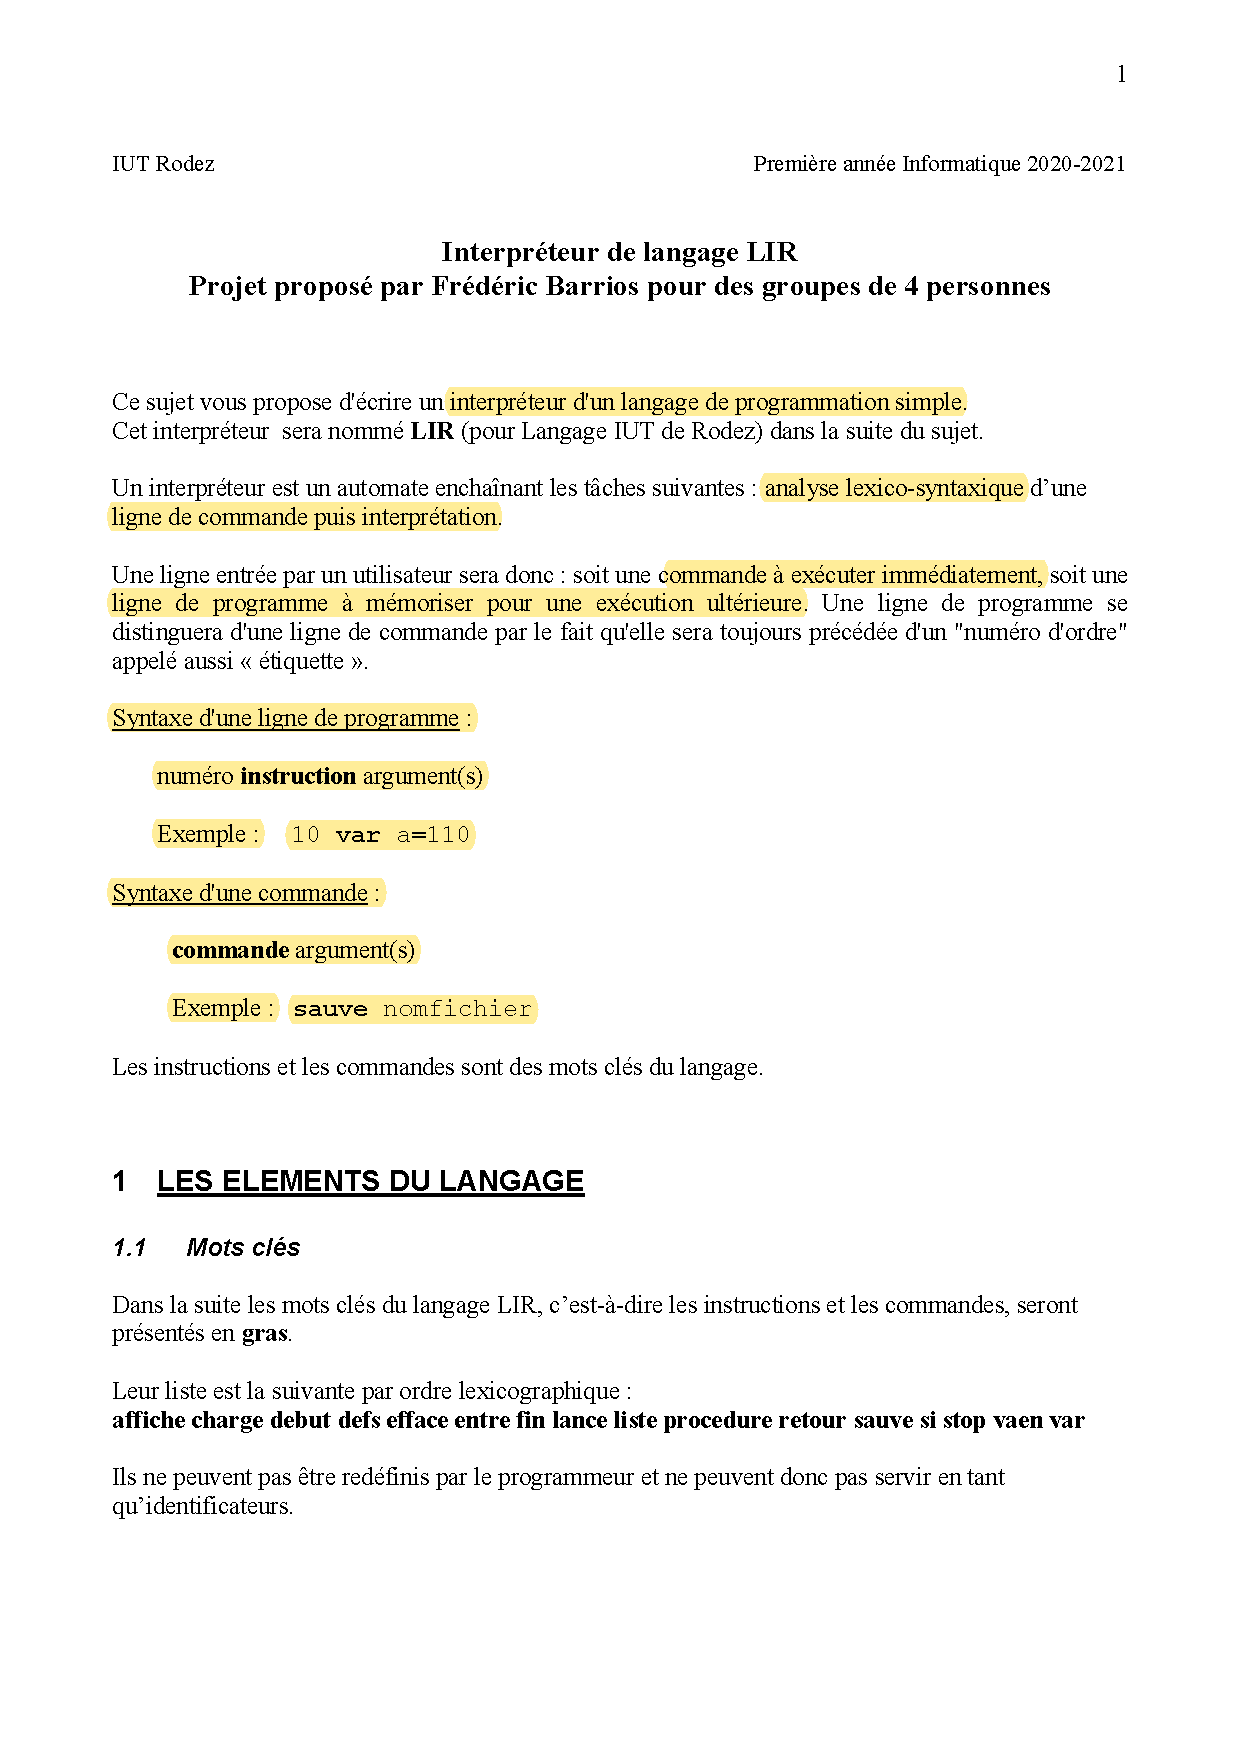
\includepdf[pages=-]{fichiers/BarriosInterpreteurLIR2021}

\end{document}